% COMP90051 Group 51 — Research Report
% Tennis Momentum. 4 pages max, 10pt, single column, A4, margins 1.5–2cm.
% Compile: pdflatex report.tex   (run twice for references)
%
% DRAFT STATUS: all prose is final. The ONLY things to replace are the numbers
% in the Results tables/figures (marked \ph{...}) and the two figure images,
% which report/make_figures.py generates from results/*.json after you run the
% experiments. Search this file for "\ph{" and "FIGURE PLACEHOLDER".
\documentclass[10pt,a4paper]{article}
\usepackage[margin=1.8cm]{geometry}
\usepackage[T1]{fontenc}
\usepackage{times}
\usepackage{amsmath}
\usepackage{booktabs}
\usepackage{graphicx}
\usepackage{caption}
\usepackage{subcaption}
\usepackage[hidelinks]{hyperref}
\usepackage{xcolor}
\usepackage{titlesec}
\usepackage{enumitem}

% Compact spacing to fit four pages.
\titlespacing*{\section}{0pt}{1.4ex plus .2ex}{0.6ex}
\titlespacing*{\subsection}{0pt}{0.9ex plus .2ex}{0.4ex}
\titleformat{\section}{\normalfont\large\bfseries}{\thesection}{0.6em}{}
\titleformat{\subsection}{\normalfont\normalsize\bfseries}{\thesubsection}{0.5em}{}
\setlength{\parskip}{0.3ex}
\setlength{\parindent}{1.2em}
\captionsetup{font=small,skip=3pt}
\setlist{nosep,leftmargin=1.4em}
\pagestyle{empty}

% Placeholder for a result you must fill in from results/*.json.
\newcommand{\ph}[1]{\textcolor{red}{#1}}

\begin{document}

\begin{center}
  {\large\bfseries Does momentum have a measurable effect on the next point in a tennis match?}\\[0.3ex]
  {\small COMP90051 Statistical Machine Learning --- Group 51\\
  Benjamin Morrison (\ph{ID}), Dev Karan Singh (\ph{ID}), Faisal Abdullah Khan (\ph{ID})}
\end{center}
\vspace{-0.5ex}

\section{Introduction}
The obvious prediction task on point-by-point tennis data is ``who wins the next
point''. That task is trivially confounded and not our research question. Service
alternates game by game, and the stronger player wins more points, so apparent
``streaks'' arise even when every point is independent: ``won the last three
points'' frequently means only ``is serving this game'' or ``is the better
player''. We therefore ask a falsifiable question about \emph{temporal
structure}:

\begin{quote}\itshape
Does the \emph{order} of the preceding points carry information about the winner
of the next point, \emph{beyond} what is explained by the server, the score and
pressure context, and player strength --- and if so, how many points back does
that memory extend?
\end{quote}

This cannot be answered by a feature-importance table; it requires an
experimental design with controls. We use three experiments: a \textbf{negative
(shuffle) control} that destroys point order while preserving serve-conditional
base rates, a \textbf{memory-horizon} sweep that measures predictive gain as a
function of how much in-match history each model sees on top of a fixed
pre-match base, and a \textbf{base-vs-full} comparison of every model trained
with and without any knowledge of how the match is going, which sizes the total
in-match information that momentum could at most account for. The negative
result is as informative as the positive one: if models do no better on real
data than on the order-destroyed null, momentum carries no predictive signal.

\textbf{Dataset.} Jeff Sackmann's Grand Slam point-by-point collection, covering
most main-draw singles matches at the four majors since 2011
(\url{https://github.com/JeffSackmann/tennis_slam_pointbypoint}). Each row is one
point, with the server, the point winner, set/game/point indices, running score,
and --- where available --- rally length, serve speed, and ace/winner/unforced-error
flags. After cleaning we retain 1{,}867{,}642 points across 10{,}284 matches.

\section{Literature review}
\textbf{Dataset.} The Sackmann collection \cite{sackmann} is scraped from the
official Grand Slam sites; field availability varies substantially by tournament
and year (serve speed, serve number and rally length are missing for many
matches), which shapes our feature choices.

\textbf{Is tennis memoryless?} Klaassen and Magnus \cite{klaassen2001} fit a
dynamic binary panel model to Wimbledon points and find that points are
\emph{not} perfectly independent and identically distributed, but that
deviations are small; winning the previous point has a minor positive
association with winning the next. This frames momentum as a small-effect
question where confound control is decisive, and motivates our shuffle control.

\textbf{The hot hand.} The ``hot hand'' debate originates with Gilovich, Vallone
and Tversky \cite{gilovich1985}, who argued the belief in streaks in basketball
was largely a cognitive misperception of randomness. Miller and Sanjurjo
\cite{miller2018} later showed that the standard streak estimator is itself
biased in finite samples, so na\"ive ``win-after-a-streak'' statistics overstate
reversals. Our within-match shuffle inherits the same bias, so comparing real
against shuffled performance cancels it rather than being misled by it.

\textbf{Algorithm paper (not covered in class).} Our complex model is the
Relational Recurrent Neural Network of Santoro et al. \cite{santoro2018}
(NeurIPS 2018). A standard LSTM --- which the subject does cover --- compresses the
past into a single hidden vector. The Relational Memory Core instead maintains a
\emph{matrix} of memory slots and, at every step, lets those slots interact
through multi-head self-attention before gating them into the next state. This
slot-to-slot self-attention is the component that distinguishes it from the
recurrent architectures taught in COMP90051 and is a post-2017 development
outside the syllabus; we use it to ask whether a model that can relate separated
past events recovers momentum structure the hand-crafted features miss.

\section{Methods}
\subsection{Preprocessing and targets}
We parse the 49 tournament files (2011--2024), normalise their column names to
one schema, decode rally length (the serve counts as shot~1; an ace is one shot,
a double fault zero), and drop points with no valid winner. Every match is then
replayed from its point winners and servers under the event's rules (scoring,
serve alternation, tiebreak format, best-of-5/3), and a match whose log breaks
them anywhere --- a game ending undecided or continuing after it is won, the
wrong server, a missing point --- is dropped (224 matches, 2.3\% of points),
because its score features would be wrong. Retirements are kept. The target is
\textbf{p1\_won}, whether player~1 wins the point; the server is an input, so
momentum is tested as information beyond serving. Men's and women's matches are
modelled separately throughout.

\subsection{Feature construction}
Each of the 109 features has a declared scope. \textbf{Pre-match} (61): from all
tour-level results since 1968, processed in playing order and joined to each
slam match strictly before it is played --- Elo (FIDE K-factors) and surface
Elo, TrueSkill with TrueSkill~2-style skill drift, opponent-adjusted serve and
return skill giving each player's expected serve-point win probability against
this opponent, rest and recent workload, career experience, recent retirements,
head-to-head share (heavy-tailed counts log-transformed), and each player's
handedness (and the server's).
\textbf{Structure} (1): who serves the point. \textbf{In-match memory} (47),
built only from earlier points of the same match: win rates over the last
$w\in\{1,3,5,10,20\}$ points, exponentially weighted win rates with decay
$d\in\{0.5,0.7,0.85,0.95\}$ (memory $\approx1/(1-d)$ points), a signed streak,
each player's serve win rate over their last 2 and 4 service games and in the
match, a Bayesian estimate of the server's serve probability (prior from
pre-match form, updated point by point), breaks, the score and pressure flags
(break, game and set point, including tiebreaks; tiebreak; first point of a
game; court side) and rally-length summaries normalised to earlier editions of
the same slam. The key feature is \textbf{surprise}: an exponentially weighted
average of (outcome $-$ pre-match expected win probability for this server
against this returner), i.e.\ momentum as a \emph{departure from what serve and
strength already predict}. Eight features that are exact sums or differences of
others (e.g.\ set difference) are computed but withheld, so the design matrix is
not singular. Leakage was tested by flipping single point outcomes: no feature at
or before the flipped point changes.

\subsection{Three algorithms of increasing complexity}
All three are evaluated on identical folds. Library code is used only for the
learners; cross-validation, tuning and metrics are our own.
\begin{itemize}
\item \textbf{Simple --- $\ell_2$ logistic regression} (scikit-learn, L-BFGS),
on features standardised with training-fold statistics. Linear in the engineered
features. Tuned: penalty $\lambda$ (men $\{0.001,0.01,0.1\}$, women
$\{0.03,0.1,0.3\}$).
\item \textbf{Medium --- gradient-boosted trees} (LightGBM; depth 3, learning
rate 0.1) on the same features, capturing interactions (e.g.\ streaks that matter
only under pressure). Tuned: number of trees (men $\{20,40,80\}$, women
$\{10,20,40\}$).
\item \textbf{Complex --- Relational RNN} \cite{santoro2018}. Instead of the
engineered memory features it reads the \emph{raw} last 60 points of the match
(who won, who served, rally length, padding flag) alongside the pre-match and
structure features, so it can find order the features never encode. Tuned:
memory slots $\{2,4,8\}$. Trained on a GPU with deterministic kernels, with
early stopping on the latest 10\% of its training matches.
\end{itemize}
Logistic regression and boosting share inputs, so a difference between them is
due to model class; the RNN changes the input representation, isolating the
value of learning from the raw sequence.

\subsection{Cross-validation (from scratch)}
Evaluation must predict the future from the past; random point-level splitting
would leak the very sequential signal under study. Matches are put in playing
order (year, then Australian Open, Roland Garros, Wimbledon, US Open, then
round) and cut into $11$ contiguous blocks of equal size; repetition~$r$ trains
on block~$r$ and tests on block~$r{+}1$, a sliding window giving $10$
repetitions. A match is wholly in train or test. Adjacent repetitions share a
block, so their scores are correlated and the error bars are somewhat optimistic.

\subsection{Nested cross-validation and tuning (from scratch)}
Inside each outer training block, matches stay in time order and the inner folds
are forward-chaining: each of $3$ inner folds trains on the earliest part of the
block and validates on the next part. Each candidate value is scored by mean
inner log-loss, the best is refit on the whole outer training block, and it is
evaluated once on the untouched outer test block. Every grid has $3$ values,
centred so that the middle one should win; we report how often each value is
chosen.

\subsection{Evaluation metrics (from scratch)}
We compute log-loss, Brier score, AUC (via the rank identity), accuracy and
calibration bins ourselves; they agree with reference implementations to within
$10^{-7}$. Log-loss and Brier are primary because the question concerns
probability quality. Comparisons between conditions on the same folds (real
vs.\ shuffled, full vs.\ base) are \emph{paired} per fold. We do not report loss
against training epochs.

\section{Results and discussion}
Log-loss differences below are paired per fold and given in units of
$10^{-4}$ (mean $\pm$ s.e.\ over the 10 folds); positive means the first-named
condition predicts better. The Relational RNN run is still in progress
(\ph{red} cells).

\subsection{R1 --- Shuffle control}
Table~\ref{tab:shuffle} compares each model on real data against the order-destroyed
null. The null is drawn with three shuffle seeds and its per-fold scores are
averaged over them; because real and shuffled data share identical folds, the
momentum signal is the \emph{paired} per-fold gain of real over null (its
standard error removes the fold-to-fold difficulty that dominates the unpaired
error bars, here $\pm10\times10^{-4}$ for men), reported with its spread across
seeds. If the gain is within its error bar, order carries no detectable
predictive information.

\begin{table}[h]
\centering\small
\caption{Real vs.\ order-shuffled data. Log-loss is the mean over 10 temporal
folds (null: mean over 3 seeds). Gain = paired per-fold log-loss improvement of
real over null ($\times10^{-4}$, $\pm$ s.e.); seed s.d.\ is its spread across
shuffle seeds.}
\label{tab:shuffle}
\begin{tabular}{llcccccc}
\toprule
Tour & Model & \multicolumn{2}{c}{Log-loss} & Gain & $t$ & Real & Seed \\
 & & real & null & ($\times10^{-4}$) & & better & s.d. \\
\midrule
Men   & Logistic reg.  & 0.6483 & 0.6484 & $+1.2\pm1.7$ & $+0.7$ & 7/10 & 1.8 \\
      & Grad.\ boosting & 0.6480 & 0.6478 & $-1.8\pm0.7$ & $-2.7$ & 3/10 & 0.5 \\
      & Relational RNN & \ph{0.000} & \ph{0.000} & \ph{$\pm$} & \ph{} & \ph{/10} & \ph{} \\
Women & Logistic reg.  & 0.6793 & 0.6793 & $+0.4\pm0.2$ & $+2.0$ & 7/10 & 0.2 \\
      & Grad.\ boosting & 0.6794 & 0.6794 & $+0.0\pm0.3$ & $+0.1$ & 4/10 & 0.3 \\
      & Relational RNN & \ph{0.000} & \ph{0.000} & \ph{$\pm$} & \ph{} & \ph{/10} & \ph{} \\
\bottomrule
\end{tabular}
\end{table}

No model gains from point order. Three of the four gains are within about
two standard errors of zero, and the largest positive one (women, logistic
regression, $+0.4\times10^{-4}$) is the size of the court-side and first-point
effects the null removes (see the caveat below), so it is not momentum. For men,
boosting is slightly \emph{better on the null} ($t=-2.7$): with a game's points
made exchangeable, the in-game score predicts the remaining points a little
better than in real play. This points away from momentum, not towards it.
Tuning was centred: the middle grid value was chosen in 9--10 of the 10 folds
for every model and tour.

\subsection{R2 --- Memory horizon}
Figure~\ref{fig:results}(a) plots the gain over the zero-history base (pre-match
and serve features only) as in-match history is added. It rises steadily, with
no plateau: at $H{=}10$ points the gain is $3.3\pm0.4$ (men, logistic
regression), at $H{=}50$ it is $4.6\pm0.6$, and the whole match gives
$7.3\pm0.7$; women follow the same shape at a slightly lower level ($6.2\pm0.6$
for the whole match). The largest single step is from 50 points to the whole
match, which adds the set and match score, each player's serve record over the
match, the Bayesian serve estimate and breaks. Recomputing every exponentially
weighted feature from only the last $H$ points lowers the middle of the curve by
about $0.5$--$1\times10^{-4}$ but leaves its shape unchanged. The useful
in-match information is therefore long-range --- how each player has served
across the match, and the scoreboard --- rather than a short burst of recent
points.

\subsection{R3 --- Base vs full}
Each model is trained twice on identical folds: a \emph{base} model given only
pre-match information and who is serving (ratings, serve/return expectations,
rest, head-to-head; no score and no earlier points), and the \emph{full} model
given every feature. Figure~\ref{fig:results}(b) shows the paired per-fold gain
of full over base: $7.3\pm0.7$ (men, logistic regression), $7.2\pm0.9$ (men,
boosting), $6.2\pm0.6$ and $5.5\pm0.5$ (women), better on all 10 folds in every
case, with AUC up by about $0.002$. This is the whole in-match signal --- score,
form and any momentum together --- and an upper bound on what momentum could
contribute. Read against R1, order accounts for none of it: the match situation
matters, but the order of points does not.

\begin{figure}[h]
\centering
\begin{subfigure}{0.62\linewidth}\centering
  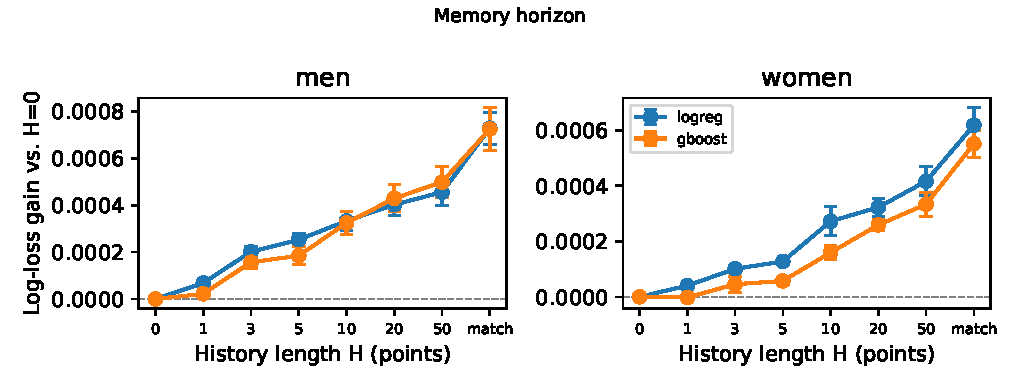
\includegraphics[width=\linewidth]{figures/memory_horizon.pdf}
  \caption{Memory horizon}
\end{subfigure}\hfill
\begin{subfigure}{0.36\linewidth}\centering
  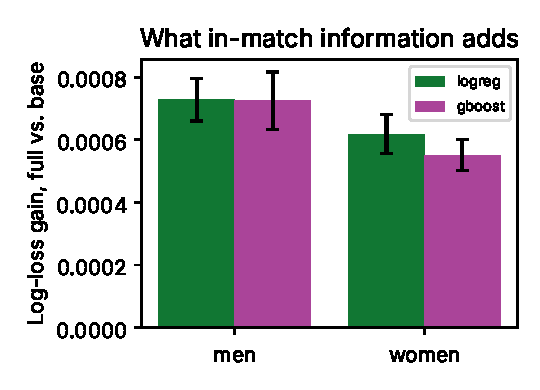
\includegraphics[width=\linewidth]{figures/base_vs_full.pdf}
  \caption{Base vs.\ full}
\end{subfigure}
\caption{(a) Paired log-loss gain over the zero-history base as history length
grows, per tour and model, with error bars over folds. (b) Paired log-loss gain
of the full model over the pre-match base model.}
\label{fig:results}
\end{figure}

\subsection{Discussion}
\textbf{Why each model behaves as it does.} Logistic regression can only express
momentum that is already encoded in the engineered windows and the surprise
feature; it is the right floor because any gain it shows is directly
interpretable as ``these summaries of the past help''. Gradient boosting adds
value only if momentum is \emph{non-linear or conditional} --- for instance if
streaks matter under break points but not otherwise --- so a boosting gain over
logistic regression localises the effect to interactions rather than to the raw
recency summaries. The Relational RNN can represent order the features never
materialise, but the momentum signal (per Klaassen and Magnus) is small and the
target is high-variance, so its large capacity is as likely to overfit as to
help; the honest expectation is that it does \emph{not} comfortably beat the
simpler models, and if it does not, that is itself evidence that hand-crafted
recency features already capture whatever short-range memory exists.

\textbf{Reading the experiments together.} The shuffle control guards against
reporting a confound as momentum: because the shuffle preserves serve-conditional
base rates, every game and set score and the match result, any real-over-null
gain cannot be explained by serving, the score or overall player strength. The
base-vs-full comparison sizes the whole in-match signal that momentum is a part
of, so the real-over-null gain can be read as a share of it rather than in
isolation, and the memory horizon locates where in the history any order effect
lives. A credible momentum claim needs a real-over-null gain that clears its
fold error \emph{and} the spread across shuffle seeds.

\textbf{Caveat: what else the null removes.} Shuffling points within a game also
moves which point is the game's first and which court each point is served
from. Two small effects that are not momentum therefore exist in the real data
but not in the null: the server wins about $0.7$ percentage points more from
the deuce court than the ad court, and about $0.8$ points less on a game's
first point than on its others (both relative to the same server in the same
set). Both are given to the models explicitly (court side, and a first-point
flag), so the real data can use them and the null cannot. Each is worth under
about $3\times10^{-5}$ in log-loss, so they put a small floor under the
real-over-null gain rather than explain it; a gain of that size or smaller
should not be read as momentum.

\textbf{Advantages and disadvantages.} The engineered-feature models are
interpretable and cheap, and their coefficients and importances say \emph{which}
horizon of history matters, but they can only find momentum we thought to encode.
The Relational RNN needs no feature guess and can model interactions among
distant points, at the cost of interpretability, higher variance, and far greater
compute --- a poor trade when the signal is weak. We chose this trio deliberately:
the simple and medium models answer ``is there linear/interaction momentum in the
features'', and the complex model guards against the charge that a null is merely
a feature-engineering failure.

\textbf{Alternatives considered.} A self-exciting point process (e.g.\ a Neural
Hawkes model) is the most natural formal model of momentum, but its event-stream
formulation does not map cleanly onto alternating-serve point data and would make
the fair, shared-fold comparison harder; we keep it as future work. A plain LSTM
was rejected as the complex model because it would not satisfy the
not-taught-in-class requirement and offers no relational mechanism over the
history. Pure ``win-after-streak'' hypothesis tests were rejected as the headline
method because of the Miller--Sanjurjo bias; we retain them only as a sanity check
whose bias the shuffle control absorbs.

\section{Conclusion}
We have framed tennis momentum as a falsifiable question --- whether point
\emph{order} predicts the next point beyond serve, score and strength, and over
what horizon --- and built a from-scratch pipeline (temporal nested
cross-validation, hand-implemented metrics, three models of increasing
complexity) whose controls make either answer defensible. No predictive
momentum is detectable above the shuffle null: the order of points adds at most
about $10^{-4}$ in log-loss, within its error bars, although the match situation
adds $5.5$--$7.3\times10^{-4}$ over pre-match information. That in-match
information is long-range --- serve form across the match and the scoreboard ---
rather than a recent run of points. \ph{Relational RNN result, which tests
whether a model reading the raw point sequence finds order the features miss.}
The methodological
contribution --- controlling for the serve, score and strength confound, and
separating order from match state --- is what separates a real answer from the
spurious streak effects that the literature warns against.

\begin{thebibliography}{9}
\small
\bibitem{sackmann} Sackmann, J. (2024). \emph{Grand Slam Point-by-Point Data}.
GitHub. \url{https://github.com/JeffSackmann/tennis_slam_pointbypoint}
\bibitem{klaassen2001} Klaassen, F.~J.~G.~M., \& Magnus, J.~R. (2001). Are points
in tennis independent and identically distributed? Evidence from a dynamic binary
panel data model. \emph{Journal of the American Statistical Association},
96(454), 500--509.
\bibitem{gilovich1985} Gilovich, T., Vallone, R., \& Tversky, A. (1985). The hot
hand in basketball: On the misperception of random sequences. \emph{Cognitive
Psychology}, 17(3), 295--314.
\bibitem{miller2018} Miller, J.~B., \& Sanjurjo, A. (2018). Surprised by the hot
hand fallacy? A truth in the law of small numbers. \emph{Econometrica}, 86(6),
2019--2047.
\bibitem{santoro2018} Santoro, A., Faulkner, R., Raposo, D., Rae, J., Chrzanowski,
M., Weber, T., Wierstra, D., Vinyals, O., Pascanu, R., \& Lillicrap, T. (2018).
Relational recurrent neural networks. \emph{Advances in Neural Information
Processing Systems (NeurIPS)}, 31.
\end{thebibliography}

\end{document}
